% Figure for the vault and the notes, section 35: straightening a graph into a slice (not from lecture).
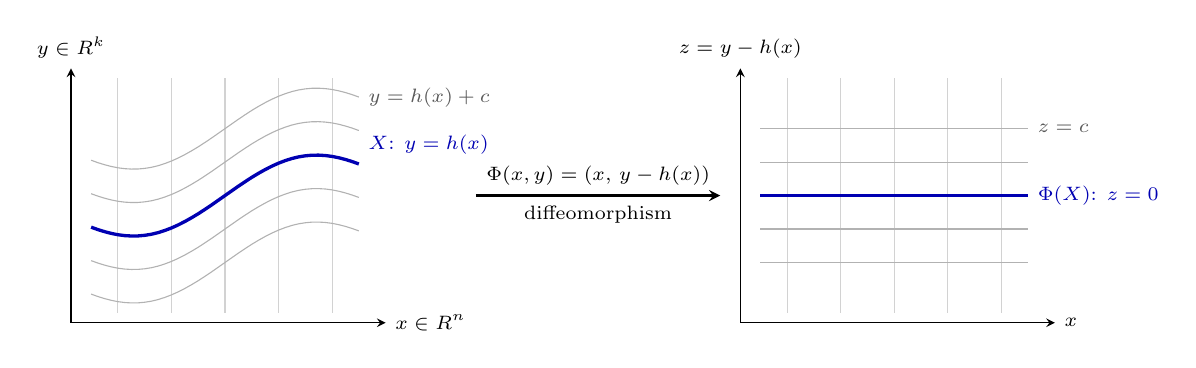
\begin{tikzpicture}[scale=0.85, >=stealth]
  \begin{scope}
    \draw[gray!35] (-1.60,-1.75) -- (-1.60,1.75);
    \draw[gray!35] (-0.80,-1.75) -- (-0.80,1.75);
    \draw[gray!35] (0.00,-1.75) -- (0.00,1.75);
    \draw[gray!35] (0.80,-1.75) -- (0.80,1.75);
    \draw[gray!35] (1.60,-1.75) -- (1.60,1.75);
    \draw[gray!60] (-2.00,-1.472) -- (-1.90,-1.508) -- (-1.80,-1.539) -- (-1.70,-1.565) -- (-1.60,-1.585) -- (-1.50,-1.598) -- (-1.40,-1.604) -- (-1.30,-1.603) -- (-1.20,-1.594) -- (-1.10,-1.578) -- (-1.00,-1.554) -- (-0.90,-1.522) -- (-0.80,-1.484) -- (-0.70,-1.439) -- (-0.60,-1.388) -- (-0.50,-1.332) -- (-0.40,-1.272) -- (-0.30,-1.207) -- (-0.20,-1.140) -- (-0.10,-1.070) -- (0.00,-1.000) -- (0.10,-0.930) -- (0.20,-0.860) -- (0.30,-0.793) -- (0.40,-0.728) -- (0.50,-0.668) -- (0.60,-0.612) -- (0.70,-0.561) -- (0.80,-0.516) -- (0.90,-0.478) -- (1.00,-0.446) -- (1.10,-0.422) -- (1.20,-0.406) -- (1.30,-0.397) -- (1.40,-0.396) -- (1.50,-0.402) -- (1.60,-0.415) -- (1.70,-0.435) -- (1.80,-0.461) -- (1.90,-0.492) -- (2.00,-0.528);
    \draw[gray!60] (-2.00,-0.972) -- (-1.90,-1.008) -- (-1.80,-1.039) -- (-1.70,-1.065) -- (-1.60,-1.085) -- (-1.50,-1.098) -- (-1.40,-1.104) -- (-1.30,-1.103) -- (-1.20,-1.094) -- (-1.10,-1.078) -- (-1.00,-1.054) -- (-0.90,-1.022) -- (-0.80,-0.984) -- (-0.70,-0.939) -- (-0.60,-0.888) -- (-0.50,-0.832) -- (-0.40,-0.772) -- (-0.30,-0.707) -- (-0.20,-0.640) -- (-0.10,-0.570) -- (0.00,-0.500) -- (0.10,-0.430) -- (0.20,-0.360) -- (0.30,-0.293) -- (0.40,-0.228) -- (0.50,-0.168) -- (0.60,-0.112) -- (0.70,-0.061) -- (0.80,-0.016) -- (0.90,0.022) -- (1.00,0.054) -- (1.10,0.078) -- (1.20,0.094) -- (1.30,0.103) -- (1.40,0.104) -- (1.50,0.098) -- (1.60,0.085) -- (1.70,0.065) -- (1.80,0.039) -- (1.90,0.008) -- (2.00,-0.028);
    \draw[gray!60] (-2.00,0.028) -- (-1.90,-0.008) -- (-1.80,-0.039) -- (-1.70,-0.065) -- (-1.60,-0.085) -- (-1.50,-0.098) -- (-1.40,-0.104) -- (-1.30,-0.103) -- (-1.20,-0.094) -- (-1.10,-0.078) -- (-1.00,-0.054) -- (-0.90,-0.022) -- (-0.80,0.016) -- (-0.70,0.061) -- (-0.60,0.112) -- (-0.50,0.168) -- (-0.40,0.228) -- (-0.30,0.293) -- (-0.20,0.360) -- (-0.10,0.430) -- (0.00,0.500) -- (0.10,0.570) -- (0.20,0.640) -- (0.30,0.707) -- (0.40,0.772) -- (0.50,0.832) -- (0.60,0.888) -- (0.70,0.939) -- (0.80,0.984) -- (0.90,1.022) -- (1.00,1.054) -- (1.10,1.078) -- (1.20,1.094) -- (1.30,1.103) -- (1.40,1.104) -- (1.50,1.098) -- (1.60,1.085) -- (1.70,1.065) -- (1.80,1.039) -- (1.90,1.008) -- (2.00,0.972);
    \draw[gray!60] (-2.00,0.528) -- (-1.90,0.492) -- (-1.80,0.461) -- (-1.70,0.435) -- (-1.60,0.415) -- (-1.50,0.402) -- (-1.40,0.396) -- (-1.30,0.397) -- (-1.20,0.406) -- (-1.10,0.422) -- (-1.00,0.446) -- (-0.90,0.478) -- (-0.80,0.516) -- (-0.70,0.561) -- (-0.60,0.612) -- (-0.50,0.668) -- (-0.40,0.728) -- (-0.30,0.793) -- (-0.20,0.860) -- (-0.10,0.930) -- (0.00,1.000) -- (0.10,1.070) -- (0.20,1.140) -- (0.30,1.207) -- (0.40,1.272) -- (0.50,1.332) -- (0.60,1.388) -- (0.70,1.439) -- (0.80,1.484) -- (0.90,1.522) -- (1.00,1.554) -- (1.10,1.578) -- (1.20,1.594) -- (1.30,1.603) -- (1.40,1.604) -- (1.50,1.598) -- (1.60,1.585) -- (1.70,1.565) -- (1.80,1.539) -- (1.90,1.508) -- (2.00,1.472);
    \draw[very thick, blue!70!black] (-2.00,-0.472) -- (-1.90,-0.508) -- (-1.80,-0.539) -- (-1.70,-0.565) -- (-1.60,-0.585) -- (-1.50,-0.598) -- (-1.40,-0.604) -- (-1.30,-0.603) -- (-1.20,-0.594) -- (-1.10,-0.578) -- (-1.00,-0.554) -- (-0.90,-0.522) -- (-0.80,-0.484) -- (-0.70,-0.439) -- (-0.60,-0.388) -- (-0.50,-0.332) -- (-0.40,-0.272) -- (-0.30,-0.207) -- (-0.20,-0.140) -- (-0.10,-0.070) -- (0.00,0.000) -- (0.10,0.070) -- (0.20,0.140) -- (0.30,0.207) -- (0.40,0.272) -- (0.50,0.332) -- (0.60,0.388) -- (0.70,0.439) -- (0.80,0.484) -- (0.90,0.522) -- (1.00,0.554) -- (1.10,0.578) -- (1.20,0.594) -- (1.30,0.603) -- (1.40,0.604) -- (1.50,0.598) -- (1.60,0.585) -- (1.70,0.565) -- (1.80,0.539) -- (1.90,0.508) -- (2.00,0.472);
    \draw[->] (-2.3,-1.9) -- (2.4,-1.9) node[right, font=\scriptsize] {$x \in \mathbb{R}^n$};
    \draw[->] (-2.3,-1.9) -- (-2.3,1.9) node[above, font=\scriptsize] {$y \in \mathbb{R}^k$};
    \node[blue!70!black, font=\scriptsize, anchor=south west] at (2.0,0.47) {$X$: $y = h(x)$};
    \node[font=\scriptsize, gray!70!black, anchor=west] at (2.0,1.47) {$y = h(x) + c$};
  \end{scope}
  \draw[->, thick] (3.75,0) -- node[above, font=\scriptsize] {$\Phi(x,y) = (x,\, y - h(x))$} node[below, font=\scriptsize] {diffeomorphism} (7.4,0);
  \begin{scope}[xshift=10.0cm]
    \draw[gray!35] (-1.60,-1.75) -- (-1.60,1.75);
    \draw[gray!35] (-0.80,-1.75) -- (-0.80,1.75);
    \draw[gray!35] (0.00,-1.75) -- (0.00,1.75);
    \draw[gray!35] (0.80,-1.75) -- (0.80,1.75);
    \draw[gray!35] (1.60,-1.75) -- (1.60,1.75);
    \draw[gray!60] (-2,-1.0) -- (2,-1.0);
    \draw[gray!60] (-2,-0.5) -- (2,-0.5);
    \draw[gray!60] (-2,0.5) -- (2,0.5);
    \draw[gray!60] (-2,1.0) -- (2,1.0);
    \draw[very thick, blue!70!black] (-2,0) -- (2,0);
    \draw[->] (-2.3,-1.9) -- (2.4,-1.9) node[right, font=\scriptsize] {$x$};
    \draw[->] (-2.3,-1.9) -- (-2.3,1.9) node[above, font=\scriptsize] {$z = y - h(x)$};
    \node[blue!70!black, font=\scriptsize, anchor=west] at (2.0,0) {$\Phi(X)$: $z = 0$};
    \node[font=\scriptsize, gray!70!black, anchor=west] at (2.0,1.0) {$z = c$};
  \end{scope}
\end{tikzpicture}